\chapter{Grafi}

\section{Introduzione}

I grafi sono tra le strutture dati più generali e potenti in informatica. Modellano relazioni tra oggetti e sono alla base di innumerevoli applicazioni: reti sociali, mappe stradali, reti di computer, dipendenze tra task, circuiti elettronici, molecole chimiche, e molto altro.

In questo capitolo studieremo le definizioni formali, le rappresentazioni in memoria, e gli algoritmi fondamentali di visita e ricerca di cammini.

\section{Definizioni fondamentali}

\begin{definizione}[Grafo]
Un \textbf{grafo} $G = (V, E)$ è una coppia ordinata dove:
\begin{itemize}
    \item $V$ è un insieme finito di \textbf{vertici} (o nodi)
    \item $E \subseteq V \times V$ è un insieme di \textbf{archi} (o spigoli)
\end{itemize}
\end{definizione}

\begin{definizione}[Grafo orientato vs non orientato]
\begin{itemize}
    \item Un grafo è \textbf{orientato} (diretto) se gli archi hanno una direzione: $(u, v) \neq (v, u)$
    \item Un grafo è \textbf{non orientato} se gli archi non hanno direzione: $(u, v) = (v, u)$
\end{itemize}
\end{definizione}

\textbf{Visualizzazione:}

\begin{center}
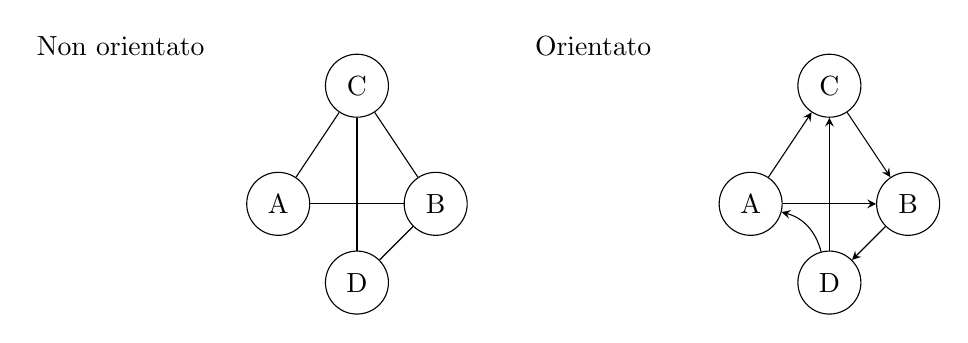
\begin{tikzpicture}[
    vertex/.style={circle, draw, minimum size=0.8cm},
    >=stealth
]
% Grafo non orientato
\node at (-2, 2) {Non orientato};
\node[vertex] (A) at (0,0) {A};
\node[vertex] (B) at (2,0) {B};
\node[vertex] (C) at (1,1.5) {C};
\node[vertex] (D) at (1,-1) {D};

\draw (A) -- (B);
\draw (A) -- (C);
\draw (B) -- (C);
\draw (B) -- (D);
\draw (C) -- (D);

% Grafo orientato
\begin{scope}[xshift=6cm]
\node at (-2, 2) {Orientato};
\node[vertex] (A2) at (0,0) {A};
\node[vertex] (B2) at (2,0) {B};
\node[vertex] (C2) at (1,1.5) {C};
\node[vertex] (D2) at (1,-1) {D};

\draw[->] (A2) -- (B2);
\draw[->] (A2) -- (C2);
\draw[->] (C2) -- (B2);
\draw[->] (B2) -- (D2);
\draw[->] (D2) -- (C2);
\draw[->] (D2) to[bend right] (A2);
\end{scope}
\end{tikzpicture}
\end{center}

\begin{definizione}[Terminologia dei grafi]
\begin{itemize}
    \item \textbf{Adiacenza}: Due vertici $u, v$ sono adiacenti se esiste un arco $(u, v) \in E$
    \item \textbf{Grado di un vertice}: Numero di archi incidenti
        \begin{itemize}
            \item Grafo orientato: \textit{grado entrante} (in-degree), \textit{grado uscente} (out-degree)
        \end{itemize}
    \item \textbf{Cammino}: Sequenza di vertici $v_0, v_1, \ldots, v_k$ tale che $(v_{i}, v_{i+1}) \in E$ per $i = 0, \ldots, k-1$
    \item \textbf{Lunghezza di un cammino}: Numero di archi nel cammino
    \item \textbf{Cammino semplice}: Cammino senza vertici ripetuti
    \item \textbf{Ciclo}: Cammino dove $v_0 = v_k$
    \item \textbf{Grafo connesso}: Esiste un cammino tra ogni coppia di vertici
    \item \textbf{Componente connessa}: Sottografo massimale connesso
    \item \textbf{Grafo pesato}: Ogni arco ha un peso $w(u, v)$
    \item \textbf{Albero}: Grafo connesso aciclico
    \item \textbf{Foresta}: Collezione di alberi disgiunti
\end{itemize}
\end{definizione}

\begin{teorema}[Somma dei gradi]
Per un grafo $G = (V, E)$:
\[
\sum_{v \in V} \deg(v) = 2|E|
\]
\end{teorema}

\begin{proof}
Ogni arco $(u, v)$ contribuisce 1 al grado di $u$ e 1 al grado di $v$, quindi contribuisce 2 alla somma totale. Sommando su tutti gli archi otteniamo $2|E|$.
\end{proof}

\begin{teorema}[Numero di archi]
In un grafo con $n$ vertici:
\begin{itemize}
    \item Grafo non orientato: al massimo $\binom{n}{2} = \frac{n(n-1)}{2}$ archi
    \item Grafo orientato: al massimo $n(n-1)$ archi
\end{itemize}
\end{teorema}

\section{Rappresentazioni dei grafi}

Esistono due rappresentazioni principali: matrice di adiacenza e lista di adiacenza.

\subsection{Matrice di adiacenza}

\begin{definizione}[Matrice di adiacenza]
Per un grafo $G = (V, E)$ con $n = |V|$ vertici, la \textbf{matrice di adiacenza} $A$ è una matrice $n \times n$ dove:
\[
A[i][j] = \begin{cases}
1 & \text{se } (i, j) \in E \\
0 & \text{altrimenti}
\end{cases}
\]

Per grafi pesati:
\[
A[i][j] = \begin{cases}
w(i, j) & \text{se } (i, j) \in E \\
\infty & \text{altrimenti}
\end{cases}
\]
\end{definizione}

\textbf{Esempio:}

\begin{center}
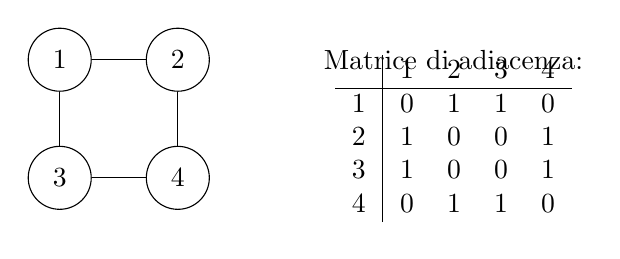
\begin{tikzpicture}[
    vertex/.style={circle, draw, minimum size=0.8cm}
]
% Grafo
\node[vertex] (1) at (0,1.5) {1};
\node[vertex] (2) at (1.5,1.5) {2};
\node[vertex] (3) at (0,0) {3};
\node[vertex] (4) at (1.5,0) {4};

\draw (1) -- (2);
\draw (1) -- (3);
\draw (2) -- (4);
\draw (3) -- (4);

% Matrice
\node at (5, 1.5) {Matrice di adiacenza:};
\node at (5, 0.5) {
\begin{tabular}{c|cccc}
  & 1 & 2 & 3 & 4 \\
\hline
1 & 0 & 1 & 1 & 0 \\
2 & 1 & 0 & 0 & 1 \\
3 & 1 & 0 & 0 & 1 \\
4 & 0 & 1 & 1 & 0 \\
\end{tabular}
};
\end{tikzpicture}
\end{center}

\textbf{Proprietà:}
\begin{itemize}
    \item Spazio: $\Theta(n^2)$
    \item Verifica se $(u, v) \in E$: $O(1)$
    \item Trovare tutti i vicini di $v$: $O(n)$
    \item Adatta per grafi densi ($|E| \approx n^2$)
    \item Per grafi non orientati, la matrice è simmetrica
\end{itemize}

\subsection{Lista di adiacenza}

\begin{definizione}[Lista di adiacenza]
Per un grafo $G = (V, E)$, la \textbf{lista di adiacenza} è un array di $|V|$ liste, dove la lista $Adj[v]$ contiene tutti i vertici adiacenti a $v$.
\end{definizione}

\textbf{Esempio (stesso grafo):}

\begin{center}
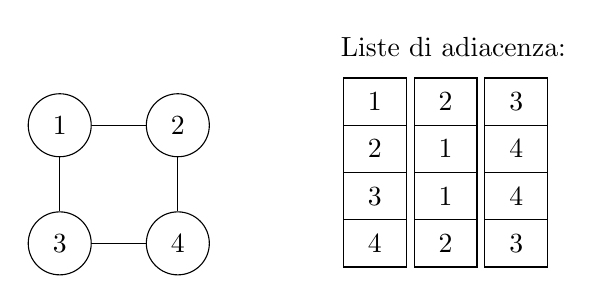
\begin{tikzpicture}[
    vertex/.style={circle, draw, minimum size=0.8cm},
    list/.style={rectangle, draw, minimum width=0.8cm, minimum height=0.6cm}
]
% Grafo
\node[vertex] (1) at (0,1.5) {1};
\node[vertex] (2) at (1.5,1.5) {2};
\node[vertex] (3) at (0,0) {3};
\node[vertex] (4) at (1.5,0) {4};

\draw (1) -- (2);
\draw (1) -- (3);
\draw (2) -- (4);
\draw (3) -- (4);

% Liste
\node at (5, 2.5) {Liste di adiacenza:};

\node[list] at (4, 1.8) {1};
\node[list] at (4.9, 1.8) {2};
\node[list] at (5.8, 1.8) {3};

\node[list] at (4, 1.2) {2};
\node[list] at (4.9, 1.2) {1};
\node[list] at (5.8, 1.2) {4};

\node[list] at (4, 0.6) {3};
\node[list] at (4.9, 0.6) {1};
\node[list] at (5.8, 0.6) {4};

\node[list] at (4, 0) {4};
\node[list] at (4.9, 0) {2};
\node[list] at (5.8, 0) {3};
\end{tikzpicture}
\end{center}

\textbf{Proprietà:}
\begin{itemize}
    \item Spazio: $\Theta(n + m)$ dove $m = |E|$
    \item Verifica se $(u, v) \in E$: $O(\deg(u))$
    \item Trovare tutti i vicini di $v$: $O(\deg(v))$
    \item Adatta per grafi sparsi ($|E| \ll n^2$)
\end{itemize}

\subsection{Confronto}

\begin{center}
\begin{tabular}{|l|c|c|}
\hline
\textbf{Operazione} & \textbf{Matrice} & \textbf{Lista} \\
\hline
Spazio & $O(n^2)$ & $O(n + m)$ \\
Verifica arco & $O(1)$ & $O(\deg(v))$ \\
Trova vicini & $O(n)$ & $O(\deg(v))$ \\
Aggiungi vertice & $O(n^2)$ & $O(1)$ \\
Aggiungi arco & $O(1)$ & $O(1)$ \\
Rimuovi arco & $O(1)$ & $O(\deg(v))$ \\
\hline
\textbf{Migliore per} & Grafi densi & Grafi sparsi \\
\hline
\end{tabular}
\end{center}

\section{Visita in ampiezza (BFS)}

\begin{definizione}[Breadth-First Search]
La \textbf{visita in ampiezza} (BFS) esplora il grafo livello per livello, partendo da un vertice sorgente $s$: prima visita tutti i vicini di $s$, poi i vicini dei vicini, e così via.
\end{definizione}

\textbf{Struttura dati:} Coda FIFO

\begin{lstlisting}[style=pseudocode]
def BFS(G, s):
    """
    Visita in ampiezza da s
    Input: grafo G, vertice sorgente s
    Output: distanze e predecessori
    Complessità: O(V + E) con liste di adiacenza
    """
    // Inizializzazione
    for ogni vertice u in G.V:
        u.colore = BIANCO
        u.distanza = ∞
        u.padre = None

    s.colore = GRIGIO
    s.distanza = 0
    s.padre = None

    Q = Queue()
    Q.enqueue(s)

    while not Q.isEmpty():
        u = Q.dequeue()

        for ogni v in G.Adj[u]:
            if v.colore == BIANCO:
                v.colore = GRIGIO
                v.distanza = u.distanza + 1
                v.padre = u
                Q.enqueue(v)

        u.colore = NERO

    return distanze, padri
\end{lstlisting}

\textbf{Colori:} L'algoritmo BFS utilizza un sistema di colorazione per tracciare lo stato di ogni vertice. Un vertice BIANCO è un vertice che non è stato ancora scoperto. Un vertice GRIGIO è stato scoperto ma non è stato completamente esplorato, ovvero sappiamo che esiste ma non abbiamo ancora visitato tutti i suoi vicini. Un vertice NERO è stato completamente esplorato: abbiamo scoperto tutti i suoi vicini e non avremo bisogno di visitarlo nuovamente.

\textbf{Esempio di esecuzione:}

\begin{center}
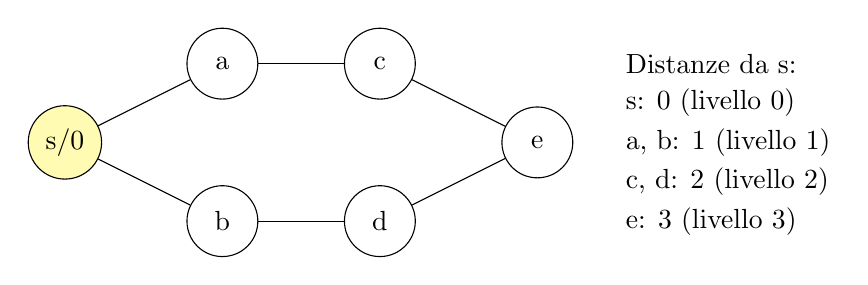
\begin{tikzpicture}[
    vertex/.style={circle, draw, minimum size=0.9cm},
    >=stealth
]
% Grafo
\node[vertex, fill=yellow!30] (s) at (0,0) {s/0};
\node[vertex] (a) at (2,1) {a};
\node[vertex] (b) at (2,-1) {b};
\node[vertex] (c) at (4,1) {c};
\node[vertex] (d) at (4,-1) {d};
\node[vertex] (e) at (6,0) {e};

\draw (s) -- (a);
\draw (s) -- (b);
\draw (a) -- (c);
\draw (b) -- (d);
\draw (c) -- (e);
\draw (d) -- (e);

% Annotazioni
\node[right] at (7, 1) {Distanze da s:};
\node[right] at (7, 0.5) {s: 0 (livello 0)};
\node[right] at (7, 0) {a, b: 1 (livello 1)};
\node[right] at (7, -0.5) {c, d: 2 (livello 2)};
\node[right] at (7, -1) {e: 3 (livello 3)};
\end{tikzpicture}
\end{center}

\begin{teorema}[Correttezza di BFS]
Sia $G = (V, E)$ un grafo e $s \in V$ il vertice sorgente. Allora:
\begin{enumerate}
    \item BFS visita tutti i vertici raggiungibili da $s$
    \item Per ogni $v$ raggiungibile da $s$, $v.distanza$ è la distanza minima da $s$ a $v$ (numero minimo di archi)
    \item L'albero dei padri BFS rappresenta i cammini minimi da $s$
\end{enumerate}
\end{teorema}

\begin{proof}[Idea]
Per induzione sulla distanza da $s$. BFS procede per livelli, quindi scopre prima tutti i vertici a distanza $k$ prima di scoprire vertici a distanza $k+1$.
\end{proof}

\textbf{Applicazioni di BFS:} L'algoritmo BFS ha numerose applicazioni pratiche e teoriche. Innanzitutto, è lo strumento ideale per trovare il cammino più breve in grafi non pesati, dove "più breve" significa il minimo numero di archi. BFS può essere utilizzato per testare se un grafo è connesso, visitando tutti i vertici a partire da un vertice iniziale e verificando se tutti sono stati raggiunti. Allo stesso modo, può essere usato per trovare tutte le componenti connesse di un grafo. Un'applicazione sofisticata è il test del bipartitismo di un grafo, che può essere fatto colorando i vertici mentre si esegue BFS. Nel contesto del web, BFS è il fondamento degli algoritmi di web crawling. Infine, BFS trova applicazione nei sistemi di raccomandazione, dove è possibile scoprire gli amici di amici seguendo i livelli della visita.

\section{Visita in profondità (DFS)}

\begin{definizione}[Depth-First Search]
La \textbf{visita in profondità} (DFS) esplora il grafo andando "in profondità" il più possibile prima di backtrackare.
\end{definizione}

\textbf{Struttura dati:} Stack (esplicito o tramite ricorsione)

\begin{lstlisting}[style=pseudocode]
def DFS(G):
    """
    Visita in profondità di tutto il grafo
    Complessità: O(V + E)
    """
    for ogni vertice u in G.V:
        u.colore = BIANCO
        u.padre = None

    tempo = 0

    for ogni vertice u in G.V:
        if u.colore == BIANCO:
            DFS_Visit(G, u)

def DFS_Visit(G, u):
    """
    Visita ricorsiva da u
    """
    tempo = tempo + 1
    u.tempo_scoperta = tempo
    u.colore = GRIGIO

    for ogni v in G.Adj[u]:
        if v.colore == BIANCO:
            v.padre = u
            DFS_Visit(G, v)

    u.colore = NERO
    tempo = tempo + 1
    u.tempo_fine = tempo
\end{lstlisting}

\textbf{Timestamp:}
\begin{itemize}
    \item $u.tempo\_scoperta$: Quando $u$ viene scoperto
    \item $u.tempo\_fine$: Quando l'esplorazione di $u$ termina
\end{itemize}

\textbf{Visualizzazione:}

\begin{center}
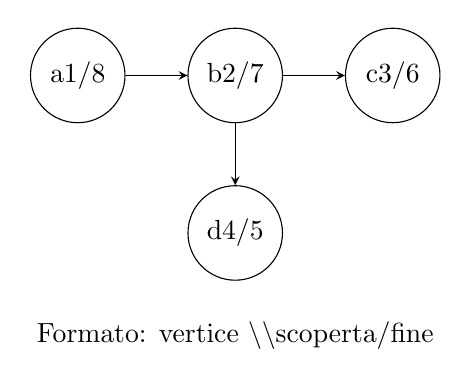
\begin{tikzpicture}[
    vertex/.style={circle, draw, minimum size=1.2cm},
    >=stealth
]
\node[vertex] (a) at (0,2) {a\\1/8};
\node[vertex] (b) at (2,2) {b\\2/7};
\node[vertex] (c) at (4,2) {c\\3/6};
\node[vertex] (d) at (2,0) {d\\4/5};

\draw[->] (a) -- (b);
\draw[->] (b) -- (c);
\draw[->] (b) -- (d);

\node[below] at (2, -1) {Formato: vertice \textbackslash\textbackslash scoperta/fine};
\end{tikzpicture}
\end{center}

\begin{teorema}[Proprietà della parentesizzazione]
Per ogni coppia di vertici $u, v$, vale esattamente una delle seguenti:
\begin{enumerate}
    \item Gli intervalli $[u.d, u.f]$ e $[v.d, v.f]$ sono disgiunti ($u$ e $v$ non sono antenati l'uno dell'altro)
    \item $[u.d, u.f] \subset [v.d, v.f]$ ($u$ è discendente di $v$)
    \item $[v.d, v.f] \subset [u.d, u.f]$ ($v$ è discendente di $u$)
\end{enumerate}
\end{teorema}

\subsection{Classificazione degli archi}

Durante DFS, ogni arco $(u, v)$ può essere classificato:

\begin{enumerate}
    \item \textbf{Arco dell'albero}: $v$ è scoperto da $u$ (parte della foresta DFS)
    \item \textbf{Arco all'indietro}: $v$ è un antenato di $u$ (crea un ciclo)
    \item \textbf{Arco in avanti}: $v$ è un discendente di $u$ (ma non nell'albero DFS)
    \item \textbf{Arco trasversale}: Tutti gli altri casi
\end{enumerate}

\begin{center}
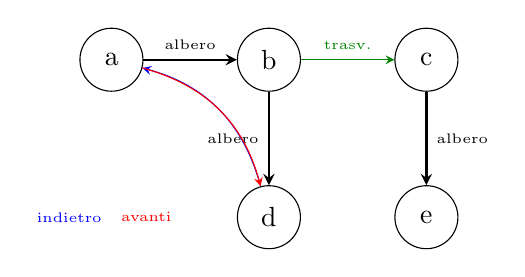
\begin{tikzpicture}[
    vertex/.style={circle, draw, minimum size=0.8cm},
    >=stealth
]
\node[vertex] (a) at (0,2) {a};
\node[vertex] (b) at (2,2) {b};
\node[vertex] (c) at (4,2) {c};
\node[vertex] (d) at (2,0) {d};
\node[vertex] (e) at (4,0) {e};

\draw[->, thick] (a) -- (b) node[midway, above] {\tiny albero};
\draw[->, thick] (b) -- (d) node[midway, left] {\tiny albero};
\draw[->, blue] (d) to[bend right] (a) node[midway, left] {\tiny indietro};
\draw[->, red] (a) to[bend left] (d) node[midway, right] {\tiny avanti};
\draw[->, green!50!black] (b) -- (c) node[midway, above] {\tiny trasv.};
\draw[->, thick] (c) -- (e) node[midway, right] {\tiny albero};
\end{tikzpicture}
\end{center}

\begin{teorema}[Rilevazione di cicli]
Un grafo orientato ha un ciclo se e solo se DFS trova un arco all'indietro.
\end{teorema}

\textbf{Applicazioni di DFS:} La visita in profondità è particolarmente utile per compiti che richiedono un'esplorazione completa della struttura del grafo. La rilevazione di cicli è una delle applicazioni più importanti: un grafo orientato ha cicli se e solo se DFS trova archi all'indietro durante l'esecuzione. L'ordinamento topologico di grafi aciclici orientati (DAG) si realizza naturalmente con DFS. Un'altra applicazione è il calcolo delle componenti fortemente connesse in grafi orientati. Nel contesto pratico, DFS è utilizzato nella risoluzione di labirinti, dove la ricerca in profondità esplora gli "agenti di scelta" (choice points) in modo sistematico fino a trovare l'uscita. Infine, DFS è fondamentale nell'analisi di dipendenze, dove i vertici rappresentano compiti o moduli e gli archi rappresentano dipendenze.

\section{Ordinamento topologico}

\begin{definizione}[Ordinamento topologico]
Un \textbf{ordinamento topologico} di un grafo orientato aciclico (DAG) è un ordinamento lineare dei vertici tale che per ogni arco $(u, v)$, $u$ appare prima di $v$ nell'ordinamento.
\end{definizione}

\begin{lstlisting}[style=pseudocode]
def OrdinamentoTopologico(G):
    """
    Ordinamento topologico usando DFS
    Precondizione: G è un DAG
    Complessità: O(V + E)
    """
    lista = []

    def DFS_Visit_Topo(u):
        u.colore = GRIGIO

        for ogni v in G.Adj[u]:
            if v.colore == BIANCO:
                DFS_Visit_Topo(v)

        u.colore = NERO
        lista.prepend(u)  // Aggiungi in testa

    for ogni vertice u in G.V:
        u.colore = BIANCO

    for ogni vertice u in G.V:
        if u.colore == BIANCO:
            DFS_Visit_Topo(u)

    return lista
\end{lstlisting}

\textbf{Esempio:}

\begin{center}
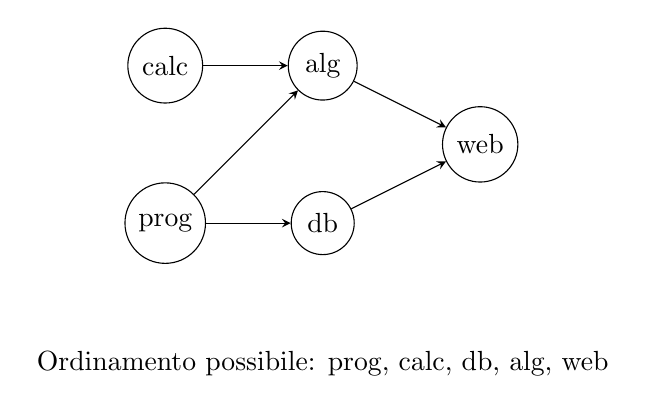
\begin{tikzpicture}[
    vertex/.style={circle, draw, minimum size=0.8cm},
    >=stealth
]
\node[vertex] (calc) at (0,2) {calc};
\node[vertex] (alg) at (2,2) {alg};
\node[vertex] (prog) at (0,0) {prog};
\node[vertex] (db) at (2,0) {db};
\node[vertex] (web) at (4,1) {web};

\draw[->] (calc) -- (alg);
\draw[->] (prog) -- (alg);
\draw[->] (prog) -- (db);
\draw[->] (alg) -- (web);
\draw[->] (db) -- (web);

\node[below] at (2, -1.5) {Ordinamento possibile: prog, calc, db, alg, web};
\end{tikzpicture}
\end{center}

\section{Cammini minimi}

\subsection{Algoritmo di Dijkstra}

L'algoritmo di Dijkstra trova i cammini minimi da una sorgente $s$ a tutti gli altri vertici in un grafo con pesi \textbf{non negativi}.

\textbf{Idea:} Espansione greedy. Manteniamo un insieme $S$ di vertici per cui conosciamo già la distanza minima. Ad ogni iterazione, aggiungiamo il vertice $u \notin S$ con distanza minima.

\begin{lstlisting}[style=pseudocode]
def Dijkstra(G, w, s):
    """
    Cammini minimi da s con pesi non negativi
    Input: grafo G, funzione peso w, sorgente s
    Output: distanze minime da s
    Complessità: O((V + E) log V) con min-heap
    """
    // Inizializzazione
    for ogni vertice v in G.V:
        v.distanza = ∞
        v.padre = None

    s.distanza = 0

    // Coda con priorità (min-heap)
    Q = MinPriorityQueue(G.V)  // priorità = distanza

    while not Q.isEmpty():
        u = Q.extractMin()

        for ogni v in G.Adj[u]:
            // Rilassamento
            if v.distanza > u.distanza + w(u, v):
                v.distanza = u.distanza + w(u, v)
                v.padre = u
                Q.decreaseKey(v, v.distanza)

    return distanze
\end{lstlisting}

\textbf{Esempio:}

\begin{center}
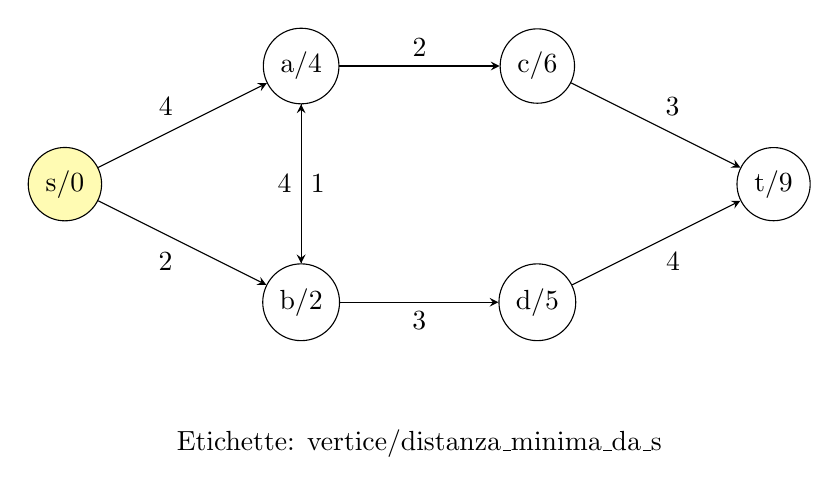
\begin{tikzpicture}[
    vertex/.style={circle, draw, minimum size=0.9cm},
    >=stealth
]
\node[vertex, fill=yellow!30] (s) at (0,0) {s/0};
\node[vertex] (a) at (3,1.5) {a/4};
\node[vertex] (b) at (3,-1.5) {b/2};
\node[vertex] (c) at (6,1.5) {c/6};
\node[vertex] (d) at (6,-1.5) {d/5};
\node[vertex] (t) at (9,0) {t/9};

\draw[->] (s) -- node[above left] {4} (a);
\draw[->] (s) -- node[below left] {2} (b);
\draw[->] (a) -- node[above] {2} (c);
\draw[->] (b) -- node[below] {3} (d);
\draw[->] (a) -- node[right] {1} (b);
\draw[->] (b) -- node[left] {4} (a);
\draw[->] (c) -- node[above right] {3} (t);
\draw[->] (d) -- node[below right] {4} (t);

\node[below] at (4.5, -3) {Etichette: vertice/distanza\_minima\_da\_s};
\end{tikzpicture}
\end{center}

\begin{teorema}[Correttezza di Dijkstra]
Se tutti i pesi sono non negativi, l'algoritmo di Dijkstra calcola correttamente le distanze minime dalla sorgente.
\end{teorema}

\begin{proof}[Idea]
Per induzione sull'insieme $S$ dei vertici processati. Quando aggiungiamo $u$ a $S$, $u.distanza$ è già il valore minimo perché tutti i cammini alternativi passano attraverso vertici non ancora in $S$, che hanno distanza $\geq u.distanza$, e tutti i pesi sono non negativi.
\end{proof}

\subsection{Algoritmo di Bellman-Ford}

Bellman-Ford gestisce anche pesi negativi e rileva cicli di peso negativo.

\begin{lstlisting}[style=pseudocode]
def BellmanFord(G, w, s):
    """
    Cammini minimi anche con pesi negativi
    Rileva cicli di peso negativo
    Complessità: O(VE)
    """
    // Inizializzazione
    for ogni vertice v in G.V:
        v.distanza = ∞
        v.padre = None

    s.distanza = 0

    // Rilassamento ripetuto
    for i = 1 to |G.V| - 1:
        for ogni arco (u, v) in G.E:
            if v.distanza > u.distanza + w(u, v):
                v.distanza = u.distanza + w(u, v)
                v.padre = u

    // Controllo cicli negativi
    for ogni arco (u, v) in G.E:
        if v.distanza > u.distanza + w(u, v):
            return "Ciclo di peso negativo rilevato"

    return distanze
\end{lstlisting}

\textbf{Complessità:} $O(VE)$ --- meno efficiente di Dijkstra, ma più generale.

\section{Tabella riassuntiva}

\begin{center}
\begin{tabular}{|l|c|c|}
\hline
\textbf{Algoritmo} & \textbf{Complessità} & \textbf{Uso} \\
\hline
BFS & $O(V + E)$ & Cammini minimi non pesati \\
DFS & $O(V + E)$ & Cicli, ordinamento topologico \\
Dijkstra & $O((V+E) \log V)$ & Cammini minimi (pesi $\geq 0$) \\
Bellman-Ford & $O(VE)$ & Cammini minimi (pesi qualsiasi) \\
\hline
\end{tabular}
\end{center}

\section{Esercizi}

\subsection{Esercizio 1}
Dimostrare che un albero con $n$ vertici ha esattamente $n-1$ archi.

\subsection{Esercizio 2}
Scrivere un algoritmo per verificare se un grafo non orientato è bipartito usando BFS.

\subsection{Esercizio 3}
Implementare l'algoritmo di Dijkstra usando una coda con priorità basata su heap.

\subsection{Esercizio 4}
Dato un grafo orientato, trovare le componenti fortemente connesse usando DFS.

\subsection{Esercizio 5}
Dimostrare che l'algoritmo di Bellman-Ford è corretto.

\section{Conclusioni}

I grafi sono strutture dati fondamentali con applicazioni vastissime:

\begin{itemize}
    \item \textbf{BFS}: Cammini minimi, livelli, bipartitismo
    \item \textbf{DFS}: Cicli, ordinamento topologico, componenti connesse
    \item \textbf{Dijkstra}: Navigatori GPS, routing di rete
    \item \textbf{Bellman-Ford}: Protocolli di routing, arbitraggio valutario
\end{itemize}

\textbf{Punti chiave:}
\begin{itemize}
    \item Liste di adiacenza per grafi sparsi, matrici per grafi densi
    \item BFS usa coda (FIFO), DFS usa stack (ricorsione)
    \item BFS trova cammini minimi non pesati
    \item Dijkstra richiede pesi non negativi
    \item Bellman-Ford gestisce pesi negativi ma è più lento
    \item Ordinamento topologico esiste solo per DAG
\end{itemize}

I grafi sono alla base di molti algoritmi avanzati: minimum spanning trees (Kruskal, Prim), flussi massimi (Ford-Fulkerson), matching, colorazione, e molto altro.
